\section*{Overview}

Persistent segment tree is what I use when the problem asks about many historical versions of an array or a frequency
structure. Instead of mutating one tree in place, every point update creates a new root while reusing all unchanged
subtrees from the previous version.

\section*{When to Use It}

Use a persistent segment tree when:

\begin{itemize}
  \item queries refer to older versions of the array,
  \item each update changes only a logarithmic number of tree nodes,
  \item prefix versions or time-stamped versions make offline queries natural.
\end{itemize}

The most common contest patterns are persistent prefix frequency trees, k-th queries on subarrays, and historical range
sums or counts.

\section*{Core Idea}

Every point update only changes the nodes on one root-to-leaf path. So instead of copying the entire segment tree, I
copy only that path and let all other pointers keep sharing the old nodes.

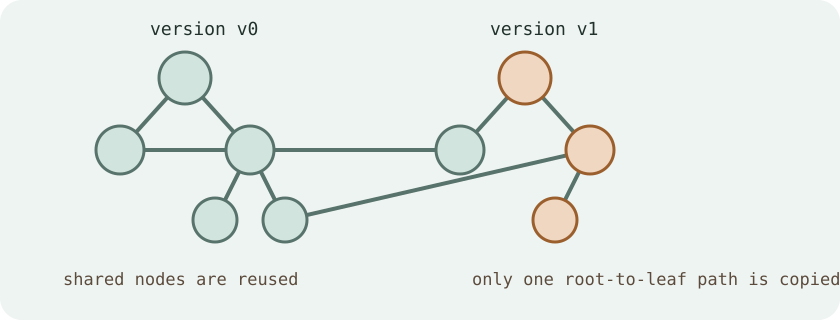
\includegraphics[width=\textwidth]{figures/version-branching.svg}

Each version is represented just by its root index or root pointer.

\section*{Key Insight}

Persistence is cheap here because the unchanged parts of the tree are still valid. Sharing them is safe because future
updates never mutate those old nodes; they create new ones instead.

\section*{Operations / Main Technique}

\begin{itemize}
  \item build an initial root,
  \item point update to produce a new root,
  \item range query on any chosen root,
  \item optionally keep many roots in a vector of versions.
\end{itemize}

\paragraph{Worked example.}
If version \(v_0\) stores the original array and I update position \(5\), the new version \(v_1\) only copies the
nodes that cover intervals containing \(5\). Everything else still points into the old tree.

\section*{Correctness Intuition}

Every version root points to a tree whose nodes exactly reflect the updates that were applied before that version was
created. Shared nodes are safe because they represent intervals untouched by the newer update. Copied nodes are exactly
the intervals whose aggregate changed.

\section*{Complexity Analysis}

\begin{itemize}
  \item one point update: \(O(\log n)\) time and \(O(\log n)\) new nodes,
  \item one range query on a chosen version: \(O(\log n)\),
  \item memory after \(q\) updates: \(O(n + q \log n)\).
\end{itemize}

\section*{Implementation}

The sample code uses an index-based node pool instead of raw pointers. It supports:

\begin{itemize}
  \item build,
  \item point update returning a new root,
  \item range-sum query on any root.
\end{itemize}

That is the smallest persistent skeleton I still trust in a contest.

\section*{Common Pitfalls}

\begin{itemize}
  \item Accidentally mutating an old node instead of cloning it.
  \item Forgetting to store every new root.
  \item Underestimating memory when the number of updates is large.
  \item Using persistence when simple offline prefix roots would already answer the problem more directly.
\end{itemize}

\section*{Variants / Extensions}

\begin{itemize}
  \item Persistent frequency tree for k-th order statistics on subarrays.
  \item Persistent lazy trees, which are possible but noticeably more fragile.
  \item Other persistent path-copy trees such as persistent treaps.
\end{itemize}

\section*{Practice Problems}

\begin{itemize}
  \item Historical point updates with range-sum queries on old versions.
  \item K-th smallest number on a subarray using prefix versions.
  \item Offline queries where every prefix version should remain accessible.
\end{itemize}

\section*{References}

\begin{itemize}
  \item \href{https://cp-algorithms.com/data_structures/segment_tree.html}{cp-algorithms: Segment Tree, persistence section}.
  \item \href{https://codeforces.com/catalog?locale=en}{Codeforces Catalog}.
  \item \href{https://github.com/kth-competitive-programming/kactl}{KACTL}.
\end{itemize}
